%%%%%%%%%%%%%%%%%%%%%%%%%%%%%%%%%%%%%%%%%
% Short Sectioned Assignment
% LaTeX Template
% Version 1.0 (5/5/12)
%
% This template has been downloaded from:
% http://www.LaTeXTemplates.com
%
% Original author:
% Frits Wenneker (http://www.howtotex.com)
%
% License:
% CC BY-NC-SA 3.0 (http://creativecommons.org/licenses/by-nc-sa/3.0/)
%
%%%%%%%%%%%%%%%%%%%%%%%%%%%%%%%%%%%%%%%%%

%----------------------------------------------------------------------------------------
%	PACKAGES AND OTHER DOCUMENT CONFIGURATIONS
%----------------------------------------------------------------------------------------

\documentclass[titlepage, paper=a4, fontsize=11pt]{scrartcl} % A4 paper and 11pt font size

\usepackage[T1]{fontenc} % Use 8-bit encoding that has 256 glyphs
\usepackage{fourier} % Use the Adobe Utopia font for the document - comment this line to return to the LaTeX default
\usepackage[english]{babel} % English language/hyphenation
\usepackage{amsmath,amsfonts,amsthm} % Math packages
\usepackage{listings}

\usepackage{lipsum} % Used for inserting dummy 'Lorem ipsum' text into the template
\usepackage{graphicx}
\usepackage{caption}
\usepackage[export]{adjustbox}


\usepackage{sectsty} % Allows customizing section commands
\allsectionsfont{\centering \normalfont\scshape} % Make all sections centered, the default font and small caps

\usepackage{fancyhdr} % Custom headers and footers
\pagestyle{fancyplain} % Makes all pages in the document conform to the custom headers and footers
\fancyhead{} % No page header - if you want one, create it in the same way as the footers below
\fancyfoot[L]{} % Empty left footer
\fancyfoot[C]{} % Empty center footer
\fancyfoot[R]{\thepage} % Page numbering for right footer
\renewcommand{\headrulewidth}{0pt} % Remove header underlines
\renewcommand{\footrulewidth}{0pt} % Remove footer underlines
\setlength{\headheight}{13.6pt} % Customize the height of the header

\numberwithin{equation}{section} % Number equations within sections (i.e. 1.1, 1.2, 2.1, 2.2 instead of 1, 2, 3, 4)
\numberwithin{figure}{section} % Number figures within sections (i.e. 1.1, 1.2, 2.1, 2.2 instead of 1, 2, 3, 4)
\numberwithin{table}{section} % Number tables within sections (i.e. 1.1, 1.2, 2.1, 2.2 instead of 1, 2, 3, 4)

\setlength\parindent{0pt} % Removes all indentation from paragraphs - comment this line for an assignment with lots of text

%----------------------------------------------------------------------------------------
%	TITLE SECTION
%----------------------------------------------------------------------------------------

\newcommand{\horrule}[1]{\rule{\linewidth}{#1}} % Create horizontal rule command with 1 argument of height

\title{	
\normalfont \normalsize 
\textsc{University of Virginia} \\ [25pt] % Your university, school and/or department name(s)
\horrule{0.5pt} \\[0.4cm] % Thin top horizontal rule
\huge ECE/CS 5565 Project 2 \\ % The assignment title
\horrule{2pt} \\[0.5cm] % Thick bottom horizontal rule
}

\renewcommand{\thefigure}{\arabic{figure}}

\author{Shawn (Shuoshuo) Chen\\sc7cq@virginia.edu} % Your name

\date{\normalsize\today} % Today's date or a custom date

\begin{document}

\maketitle % Print the title

%----------------------------------------------------------------------------------------
%	PROBLEM 1
%----------------------------------------------------------------------------------------

\section*{\textbf{Lab 1}}
\subsection*{Question 1}
\begin{figure}[!ht]
    \centering
    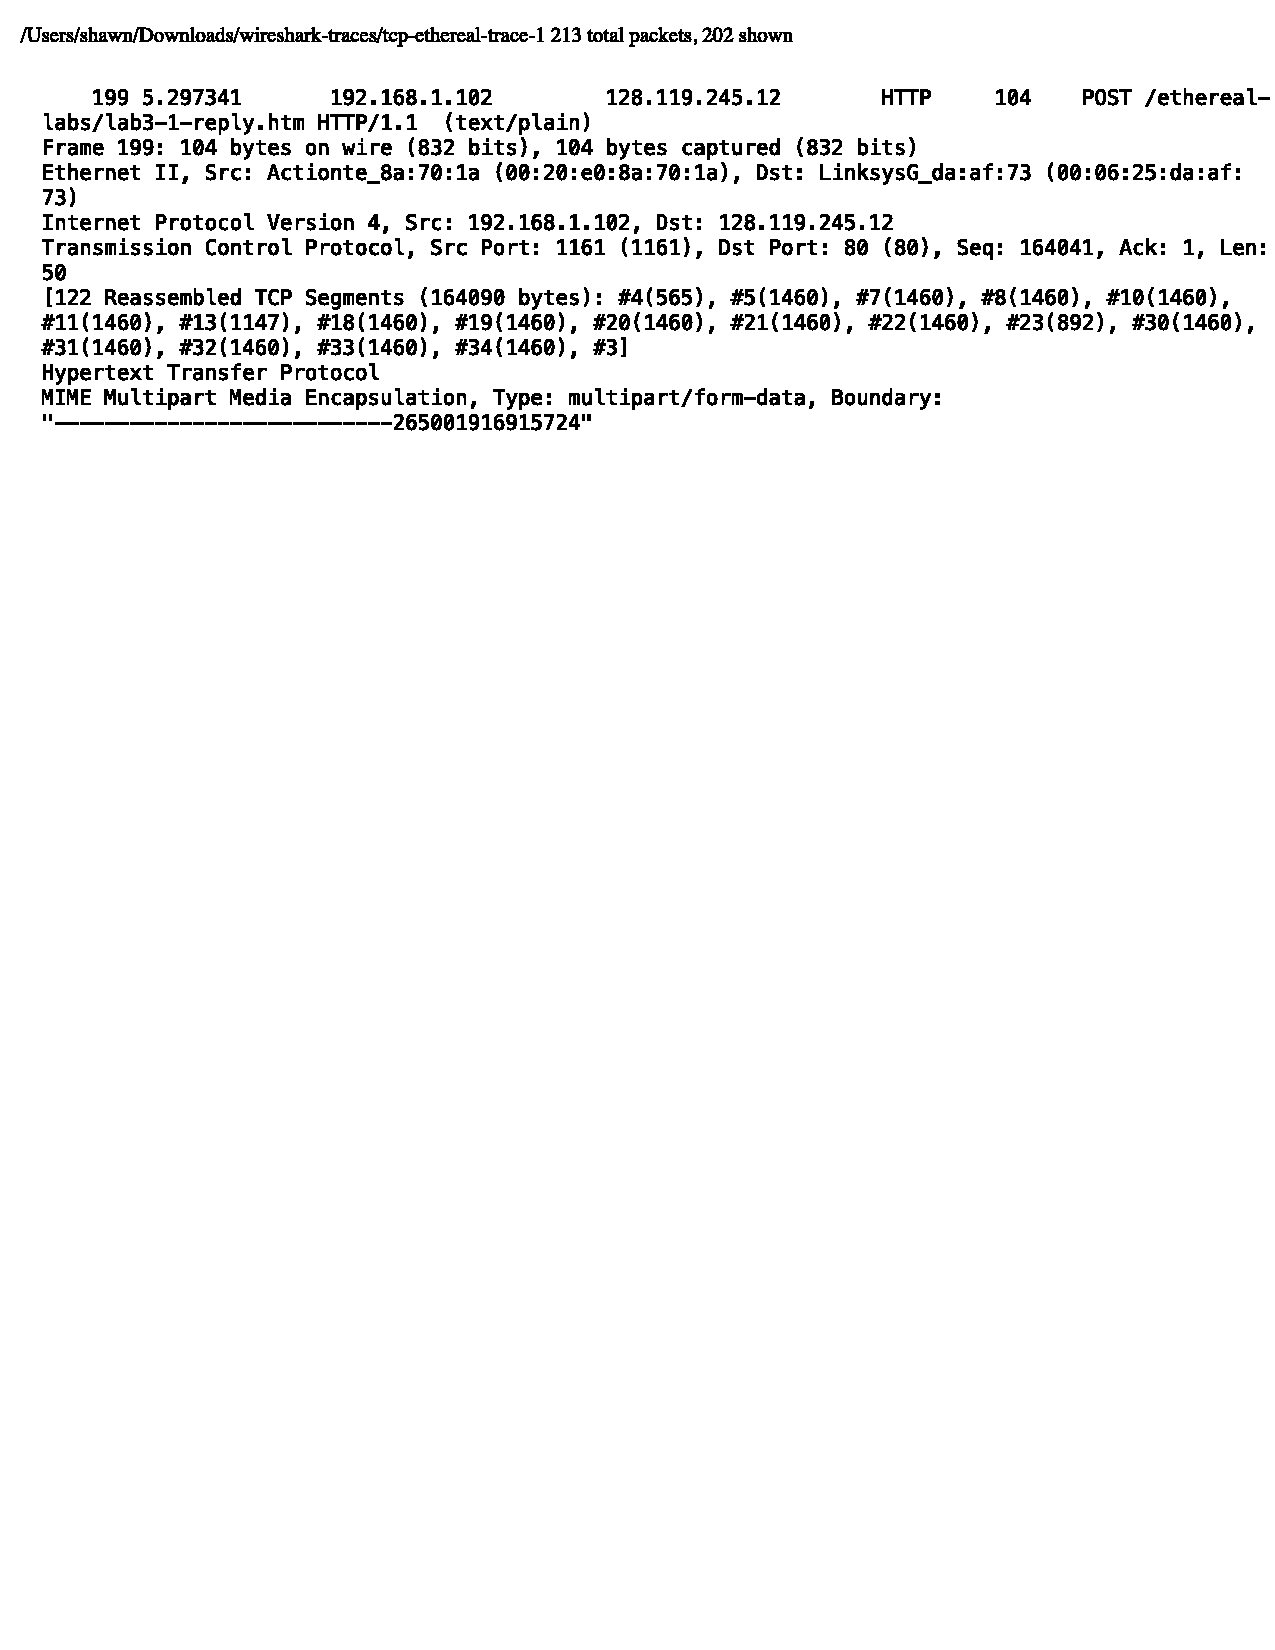
\includegraphics[width=\textwidth]{images/lab1-q1.pdf}
    \caption{HTTP POST}
    \label{fig:http-post}
\end{figure}
According to figure \ref{fig:http-post}, as displayed in the HTTP POST message, the IP addr and port of the source are: \\
192.168.1.102 and 1161. \\

\subsection*{Question 2}
From figure \ref{fig:http-post}, we can see that gaia.cs.umass.edu is sending and receiving on port 80 of IP address 128.119.245.12. \\

\subsection*{Question 3}
\begin{figure}[!ht]
    \centering
    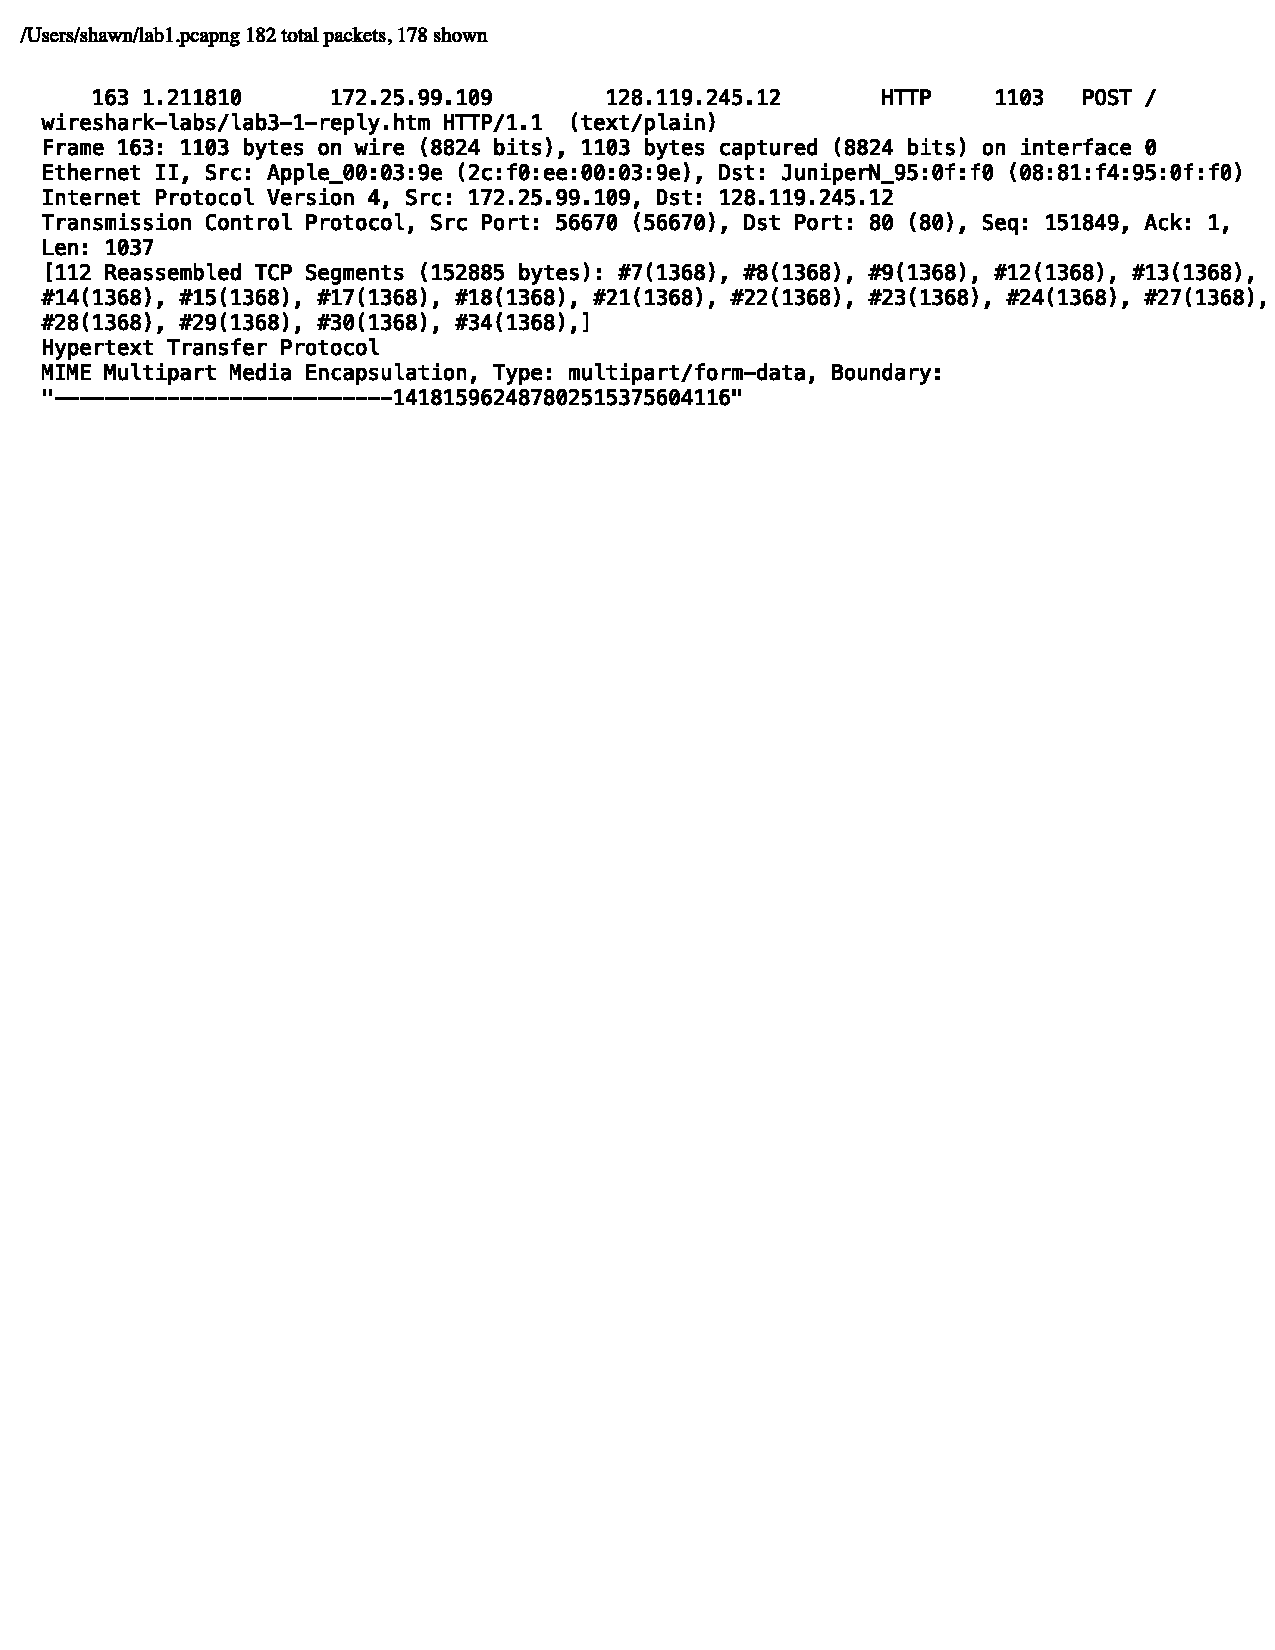
\includegraphics[width=\textwidth]{images/lab1-q3.pdf}
    \caption{HTTP POST}
    \label{fig:http-post2}
\end{figure}
According to figure \ref{fig:http-post2}, as displayed in the HTTP POST message, the IP addr and port of the source are: \\
172.25.99.109 and 56670. \\

\subsection*{Question 4}
\begin{figure}[!ht]
    \centering
    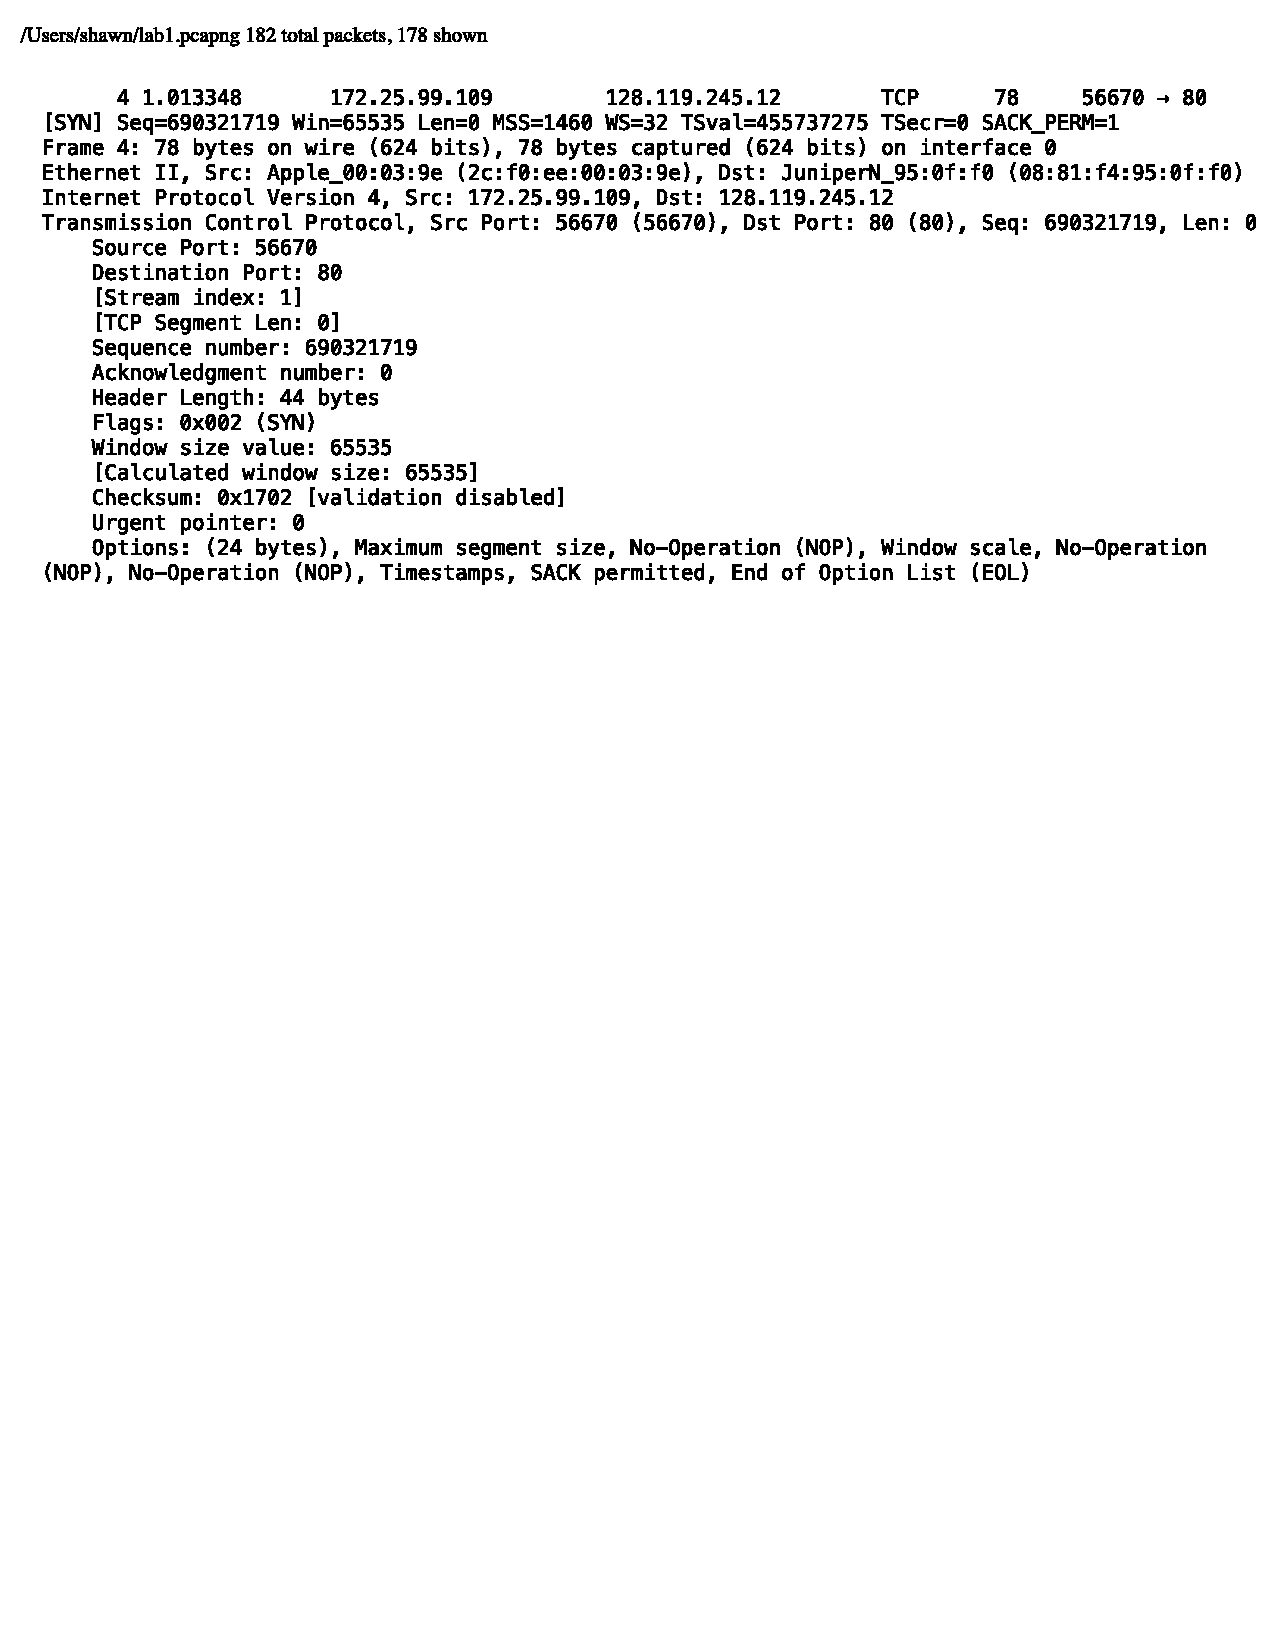
\includegraphics[width=\textwidth]{images/lab1-q4.pdf}
    \caption{TCP SYN}
    \label{fig:tcp-syn}
\end{figure}
According to figure \ref{fig:tcp-syn}, the initial sequence number is 690321719. It is the SYN bit in TCP flags field that identifies it as a SYN segment. \\

\subsection*{Question 5}
\begin{figure}[!ht]
    \centering
    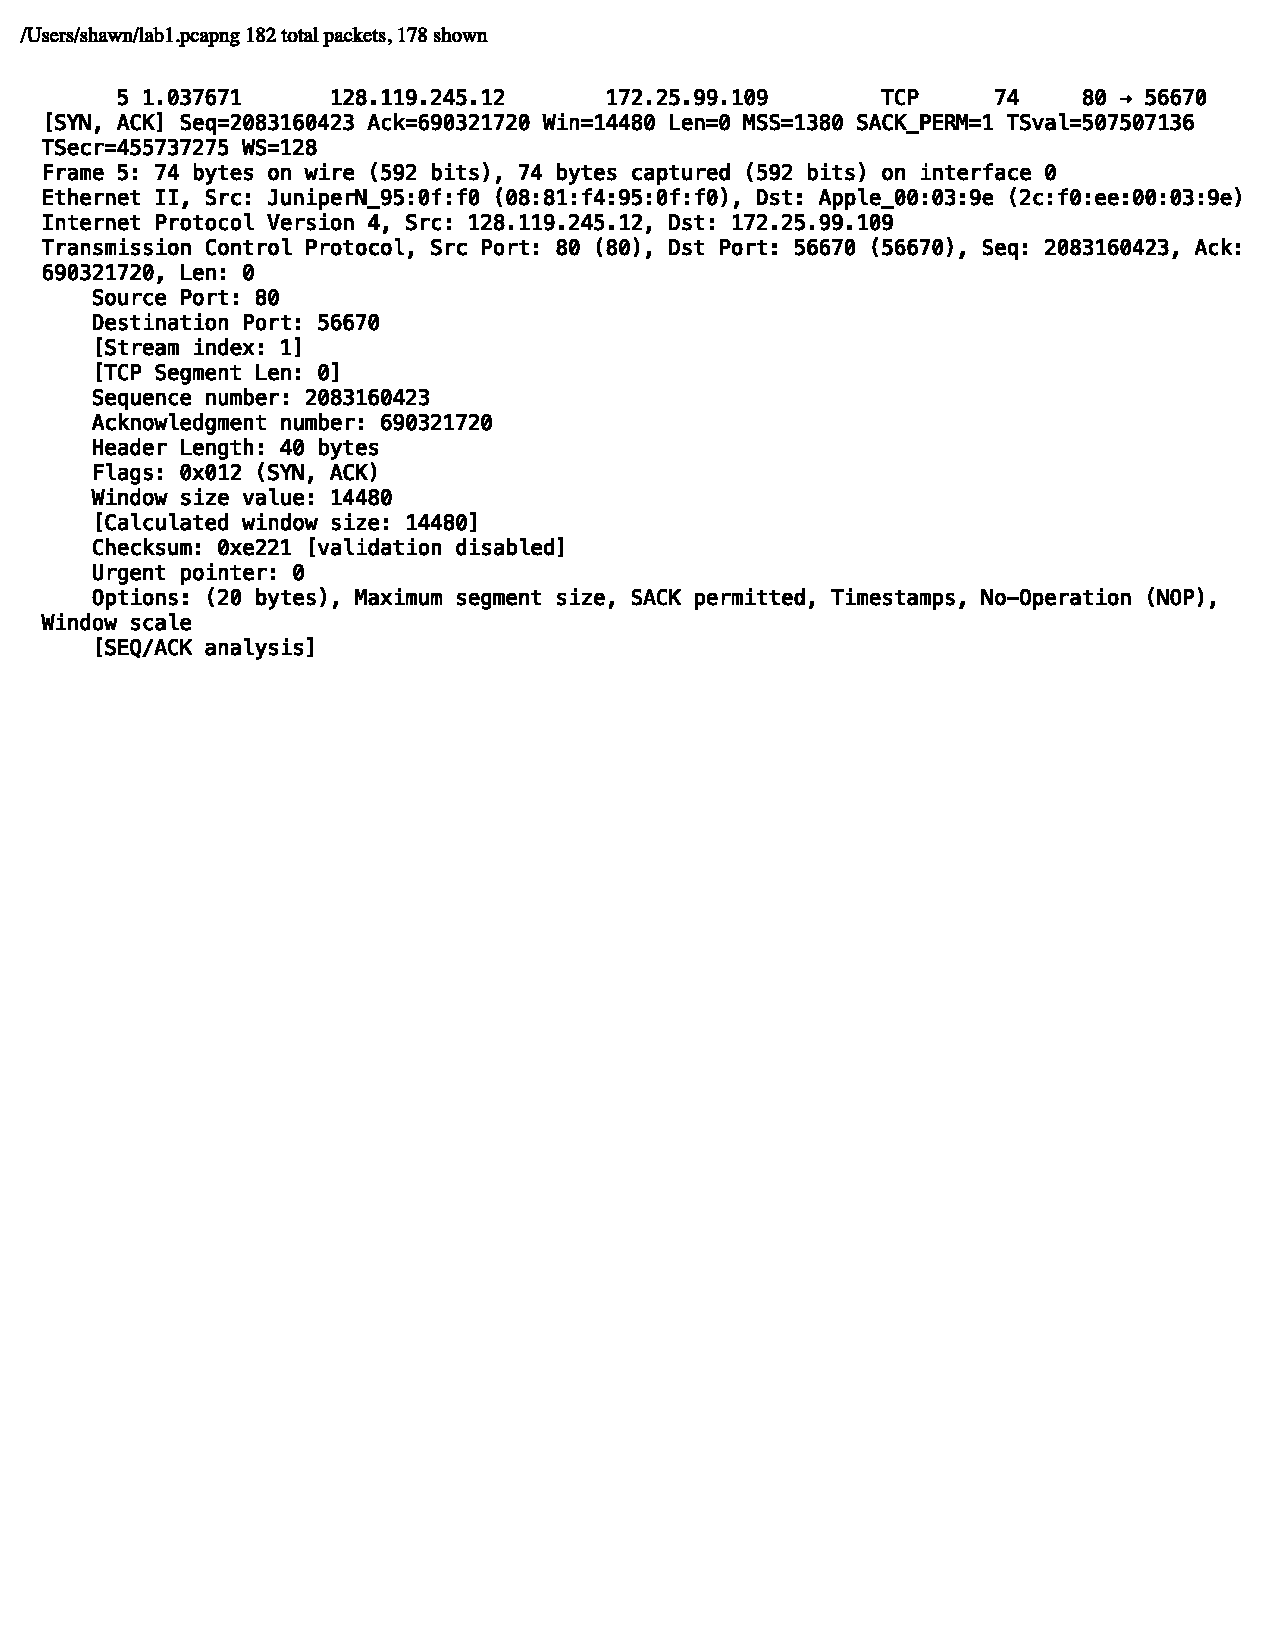
\includegraphics[width=\textwidth]{images/lab1-q5.pdf}
    \caption{TCP SYNACK}
    \label{fig:tcp-synack}
\end{figure}
According to figure \ref{fig:tcp-synack}, the sequence number in SYNACK is 2083160423. The ACK number is 690321720. gaia.cs.umass.edu randomly picks the sequence number and adds one for the received sequence number as the new ACK number. It is the SYNACK bit in TCP flags field that identifies it as a SYNACK segment. \\


\subsection*{Question 6}
\begin{figure}[!ht]
    \centering
    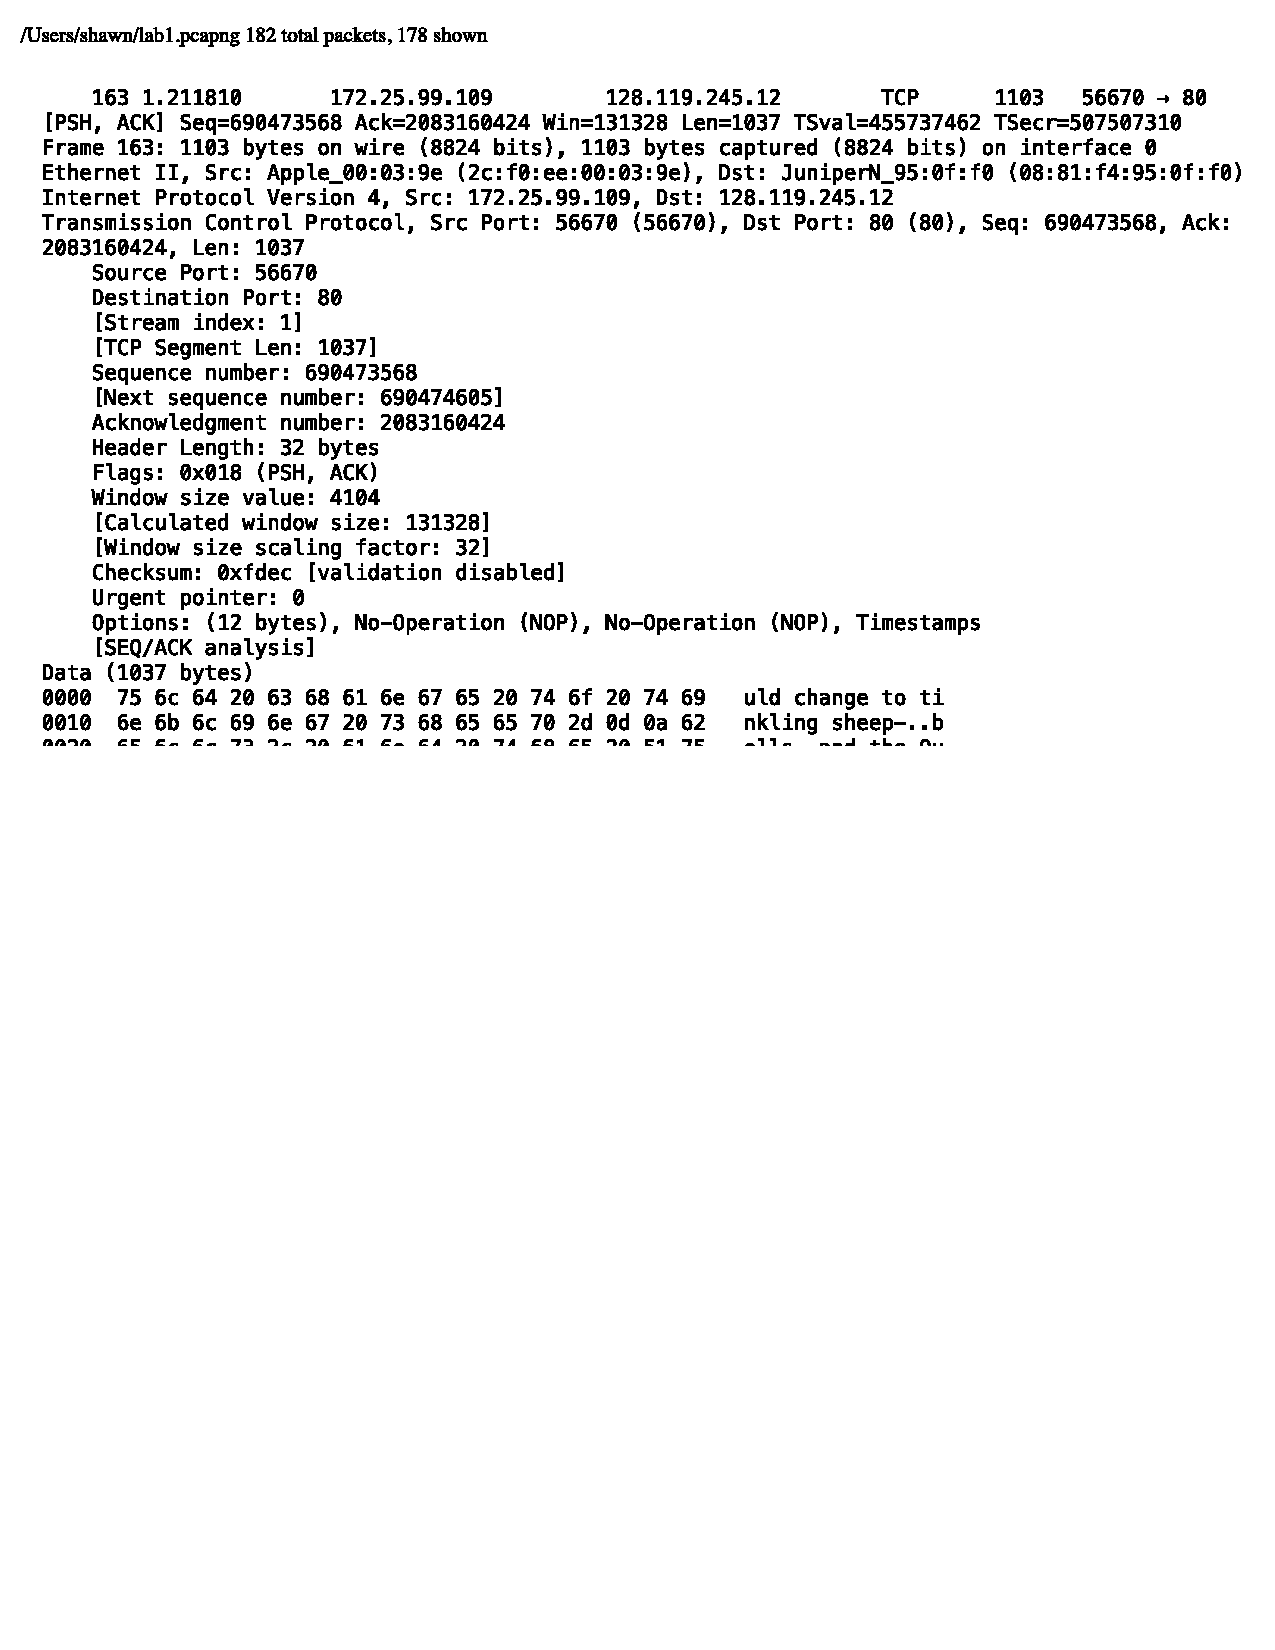
\includegraphics[width=\textwidth]{images/lab1-q6.pdf}
    \caption{HTTP POST}
    \label{fig:tcp-http-post}
\end{figure}
According to figure \ref{fig:tcp-http-post}, the sequence number contained is 690473568. \\

\subsection*{Question 8}
The first segment is 565 bytes and the rest are 1460 bytes. \\

\subsection*{Question 9}
\begin{figure}[!ht]
    \centering
    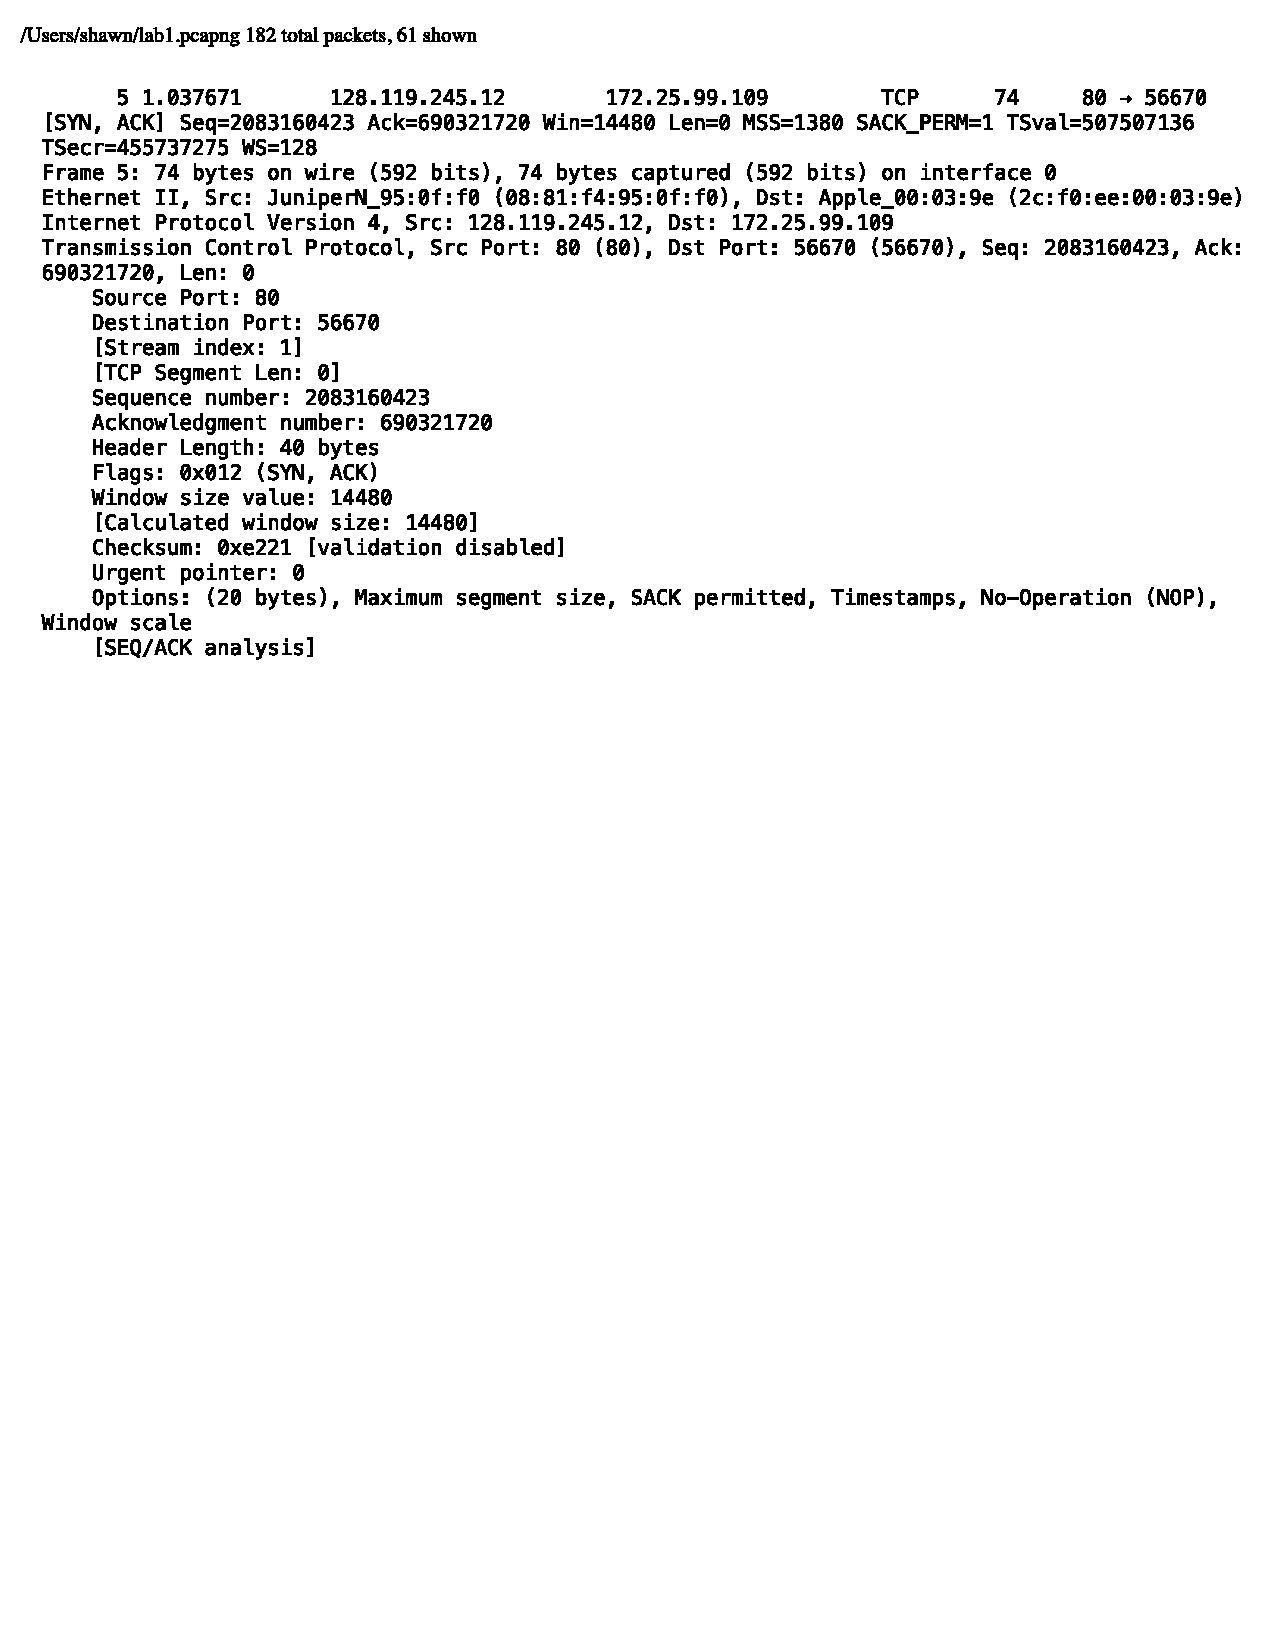
\includegraphics[width=\textwidth]{images/lab1-q9.pdf}
    \caption{TCP RECV Window}
    \label{fig:tcp-rcv-window}
\end{figure}
Going through the entire trace, the minimum advertised window size appears during the 3-way handshake phase as shown by figure \ref{fig:tcp-rcv-window}, which is 14480 bytes. Since the receving window size keeps increasing, the sender is never throttled. \\

\subsection*{Question 10}
No, there is no retransmission in the trace. I checked the sequence number in all the segments leaving my computer. It appears that the sequence number is increasing with time. I did not see any duplicate segments or sequence numbers, which indicates nothing is retransmitted. \\

\subsection*{Question 11}
\begin{figure}[!ht]
    \centering
    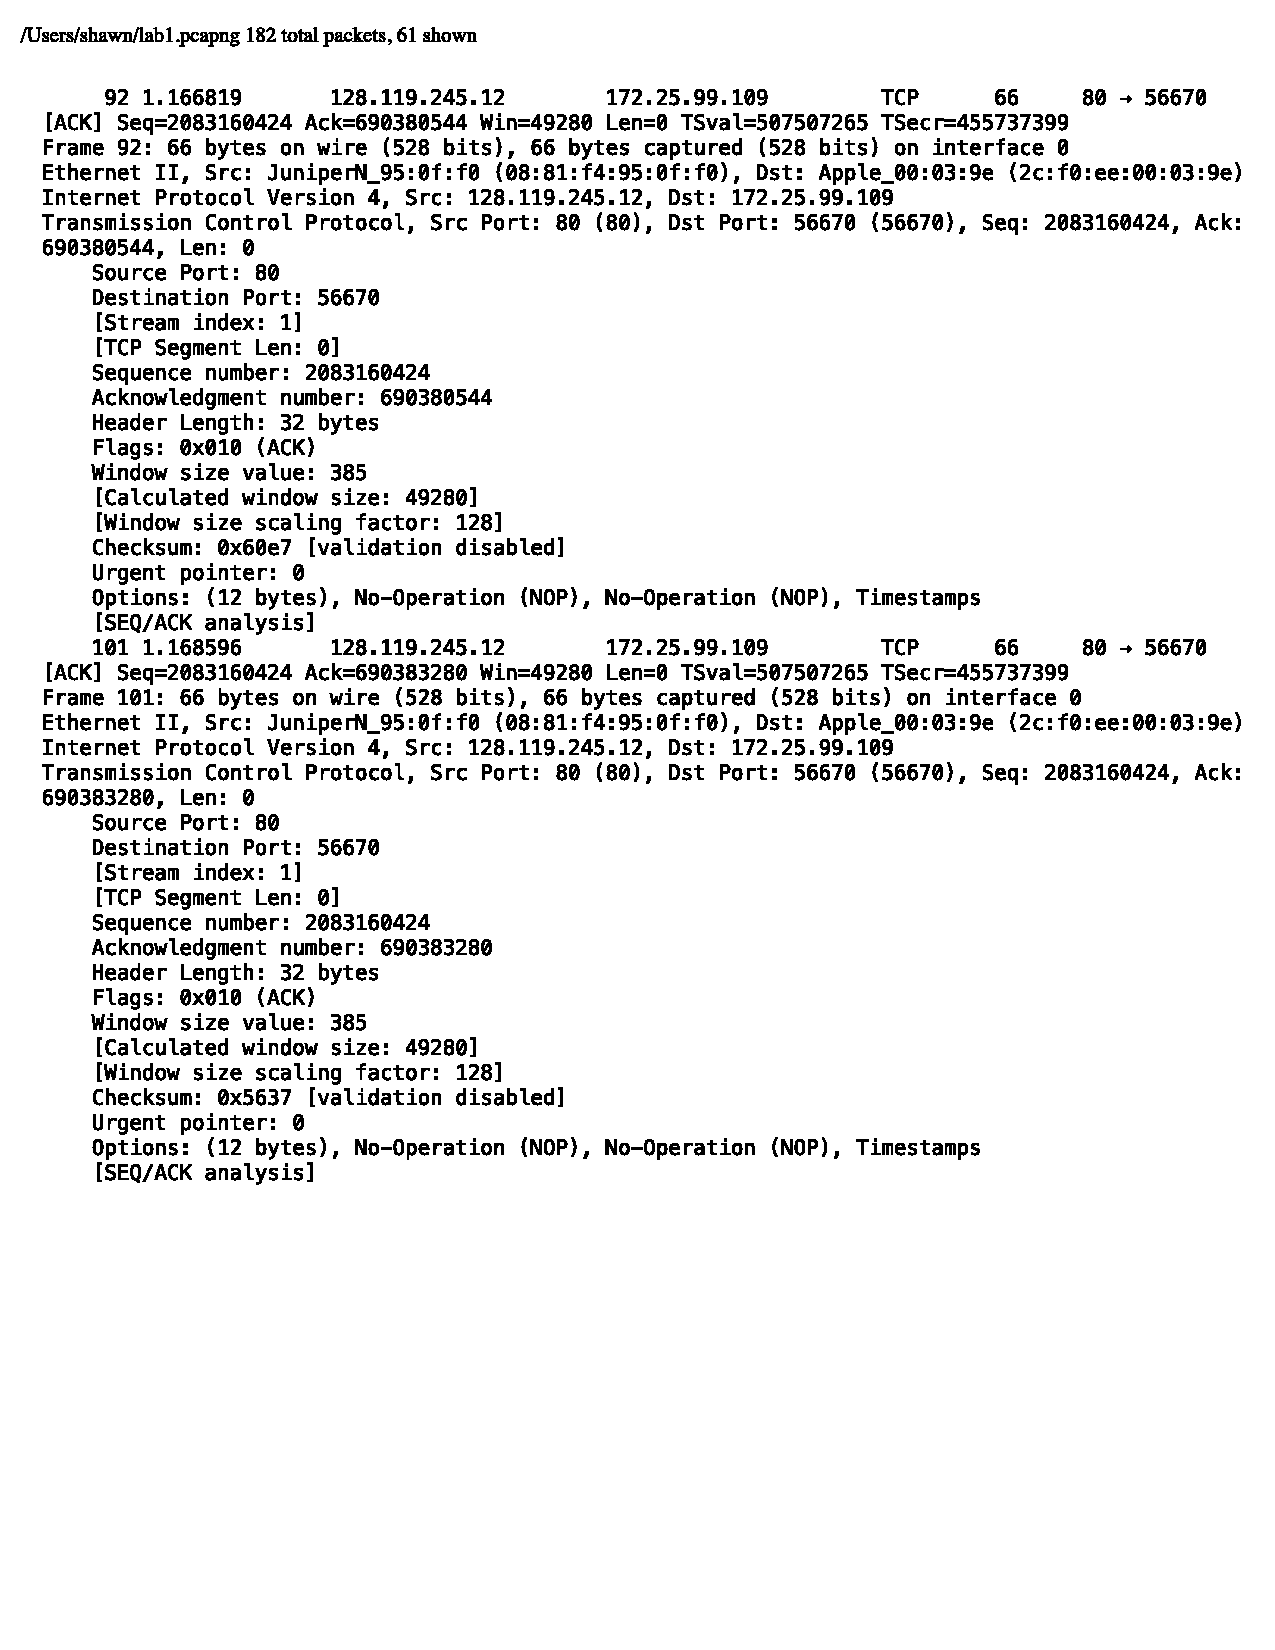
\includegraphics[width=\textwidth]{images/lab1-q11.pdf}
    \caption{TCP ACK}
    \label{fig:tcp-ack}
\end{figure}
The receiver typically acknowledges 1460 bytes in an ACK segment. But according to figure \ref{fig:tcp-ack}, the receiver acknowledged 2744 bytes, which has already exceeded the MTU. So the receiver must have ACKed two segments in one single ACK. \\

\subsection*{Question 12}
\begin{figure}[!ht]
    \centering
    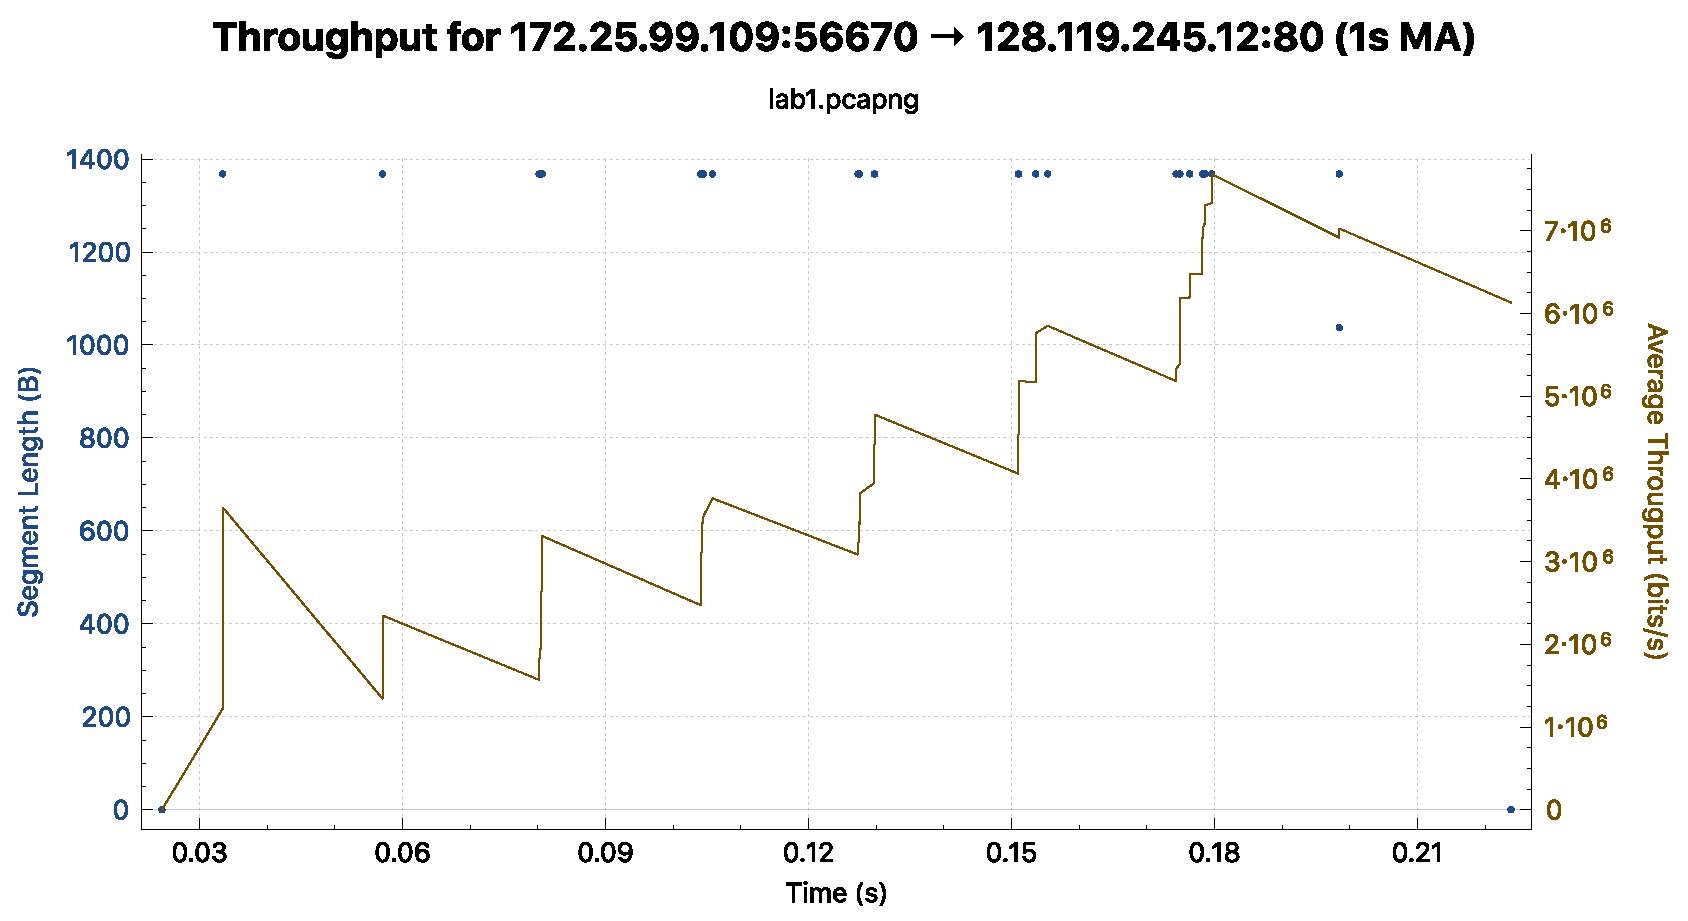
\includegraphics[width=\textwidth]{images/lab1-q12.pdf}
    \caption{TCP Throughput}
    \label{fig:tcp-thru}
\end{figure}
A high level throughput can be computed by $\tau = \frac{total size}{total time}$, where total size can be found by subtracting the sequence number $total bytes = 690474605-690321720-1=152884$ bytes. And total time can be found from the timestamp $total time = 1.237044 - 1.037671 = 0.199373 = 0.2$ seconds. So the throughput $\tau = \frac{152884}{0.2}=6.115$ Mbps. A more specific real-time throughput graph can be seen in figure \ref{fig:tcp-thru}. \\

\subsection*{Question 13}
\begin{figure}[!ht]
    \centering
    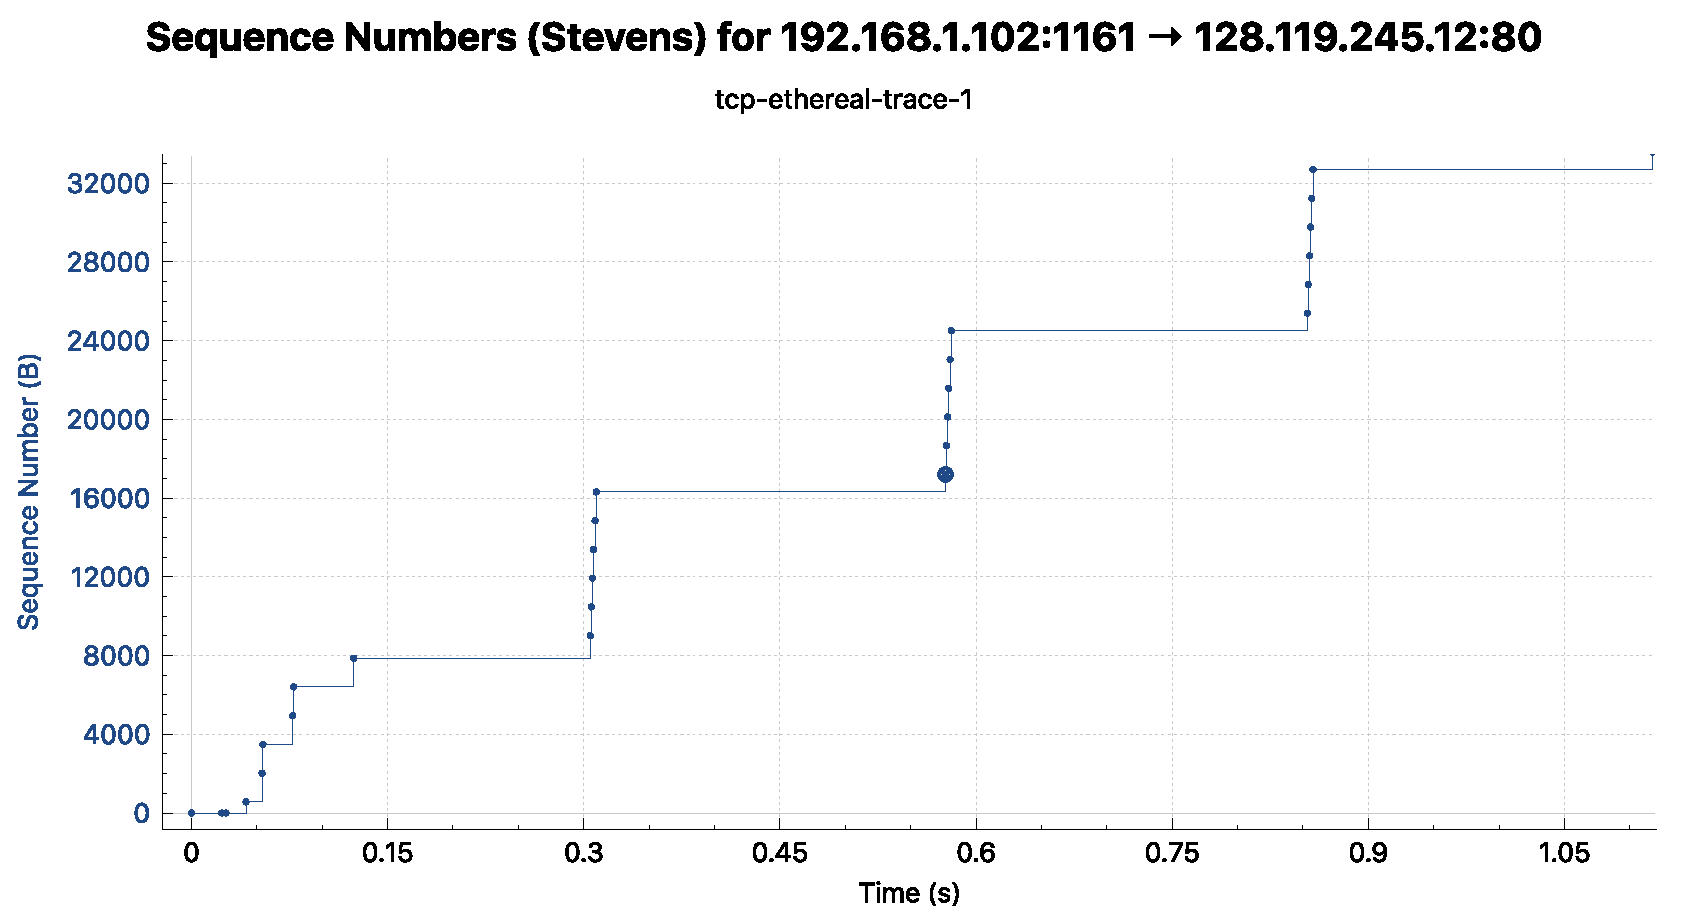
\includegraphics[width=\textwidth]{images/lab1-q13.pdf}
    \caption{TCP Slow Start}
    \label{fig:tcp-ss}
\end{figure}
According to figure \ref{fig:tcp-ss}, the number of segments sent was fixed to 6 after 0.3 seconds. So excluding the connection setup phase, the slow start phase starts from 0.03 seconds and ends by 0.3 seconds. Congestion avoidance takes over from 0.3 seconds. The difference from the ideal TCP is that the slow start did not grow exponentially (e.g. 1, 2, 4, 8, etc.). Rather, it repeated sending 2 segments twice and then sent a single outstanding segment. \\

\subsection*{Question 14}
\begin{figure}[!ht]
    \centering
    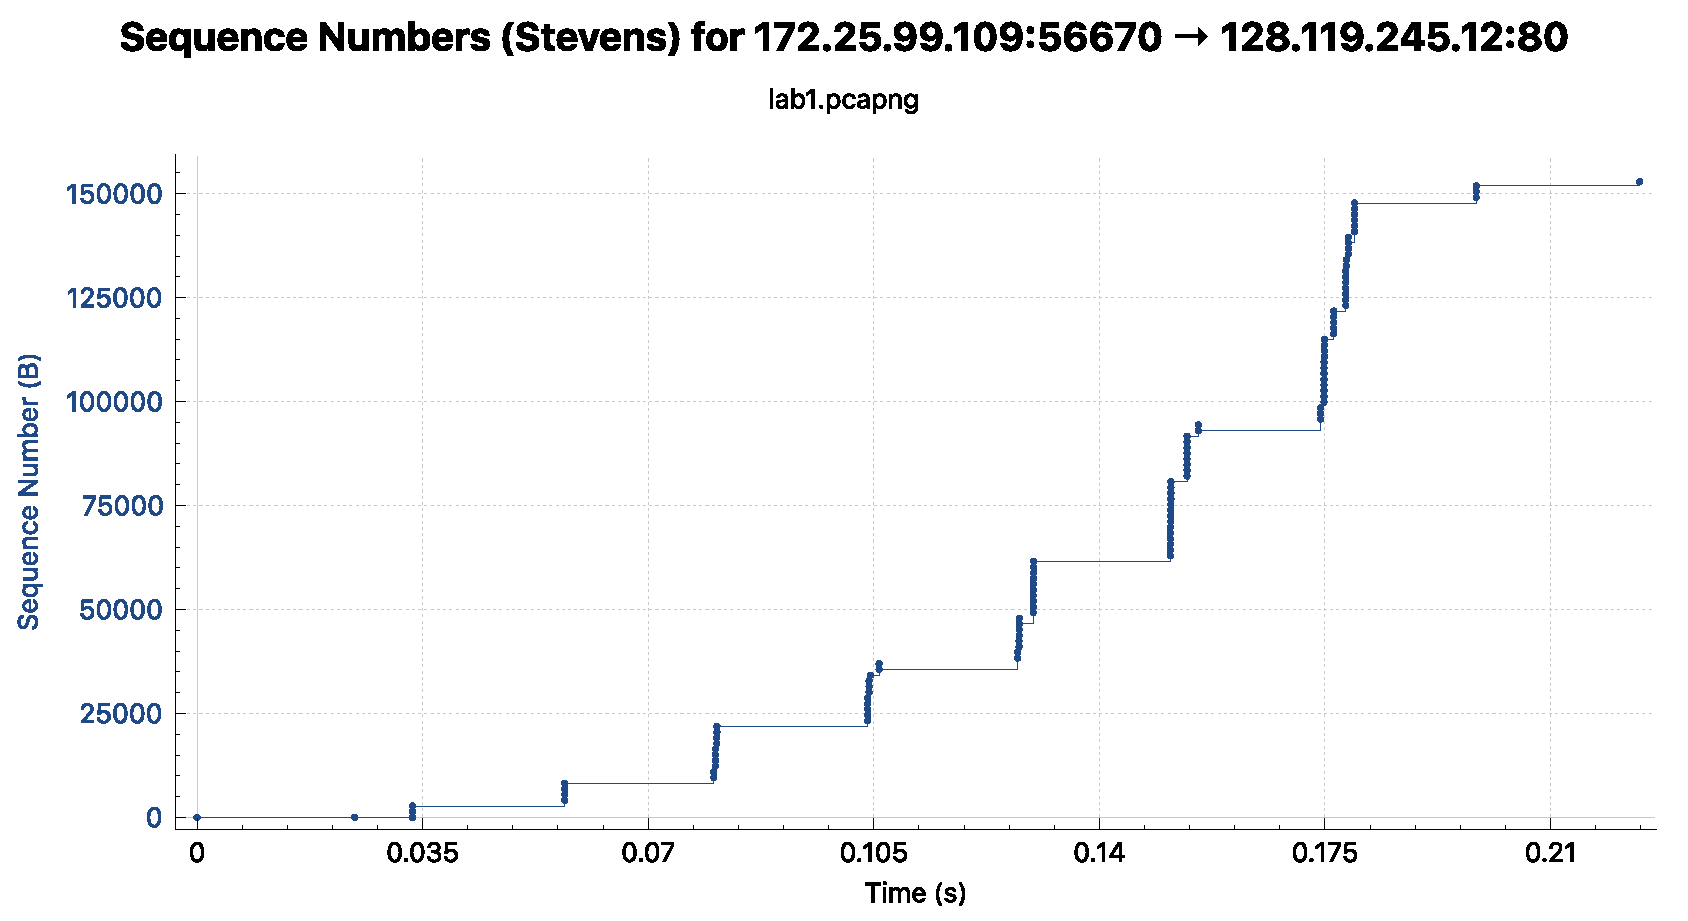
\includegraphics[width=\textwidth]{images/lab1-q14.pdf}
    \caption{TCP Slow Start}
    \label{fig:tcp-ss2}
\end{figure}
According to figure \ref{fig:tcp-ss2}, the slow start phase starts from 0.033 seconds and ends by 0.105 seconds. Congestion avoidance takes over from 0.105 seconds. The slow start phase accords with the ideal TCP in the textbook. \\




\section*{\textbf{Lab 2}}
\subsection*{Question 1}
\begin{figure}[!ht]
    \centering
    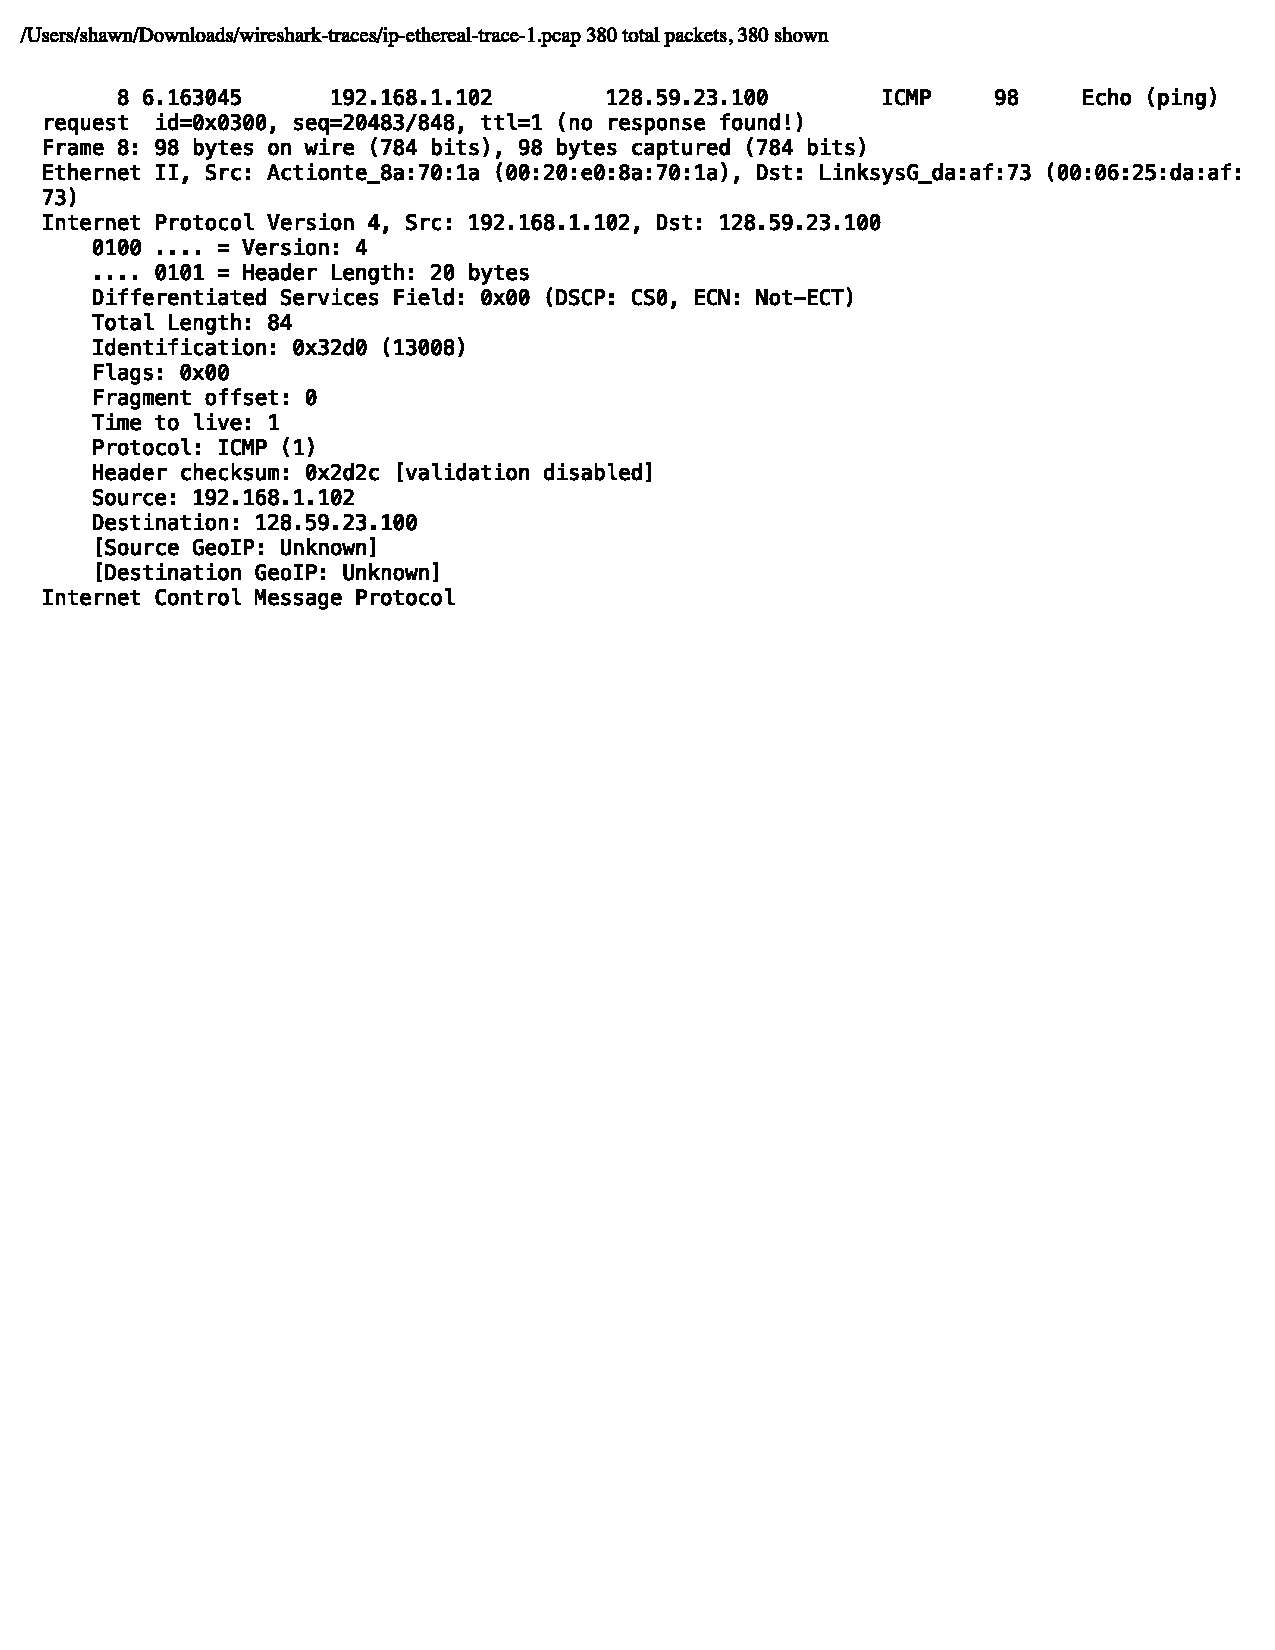
\includegraphics[width=\textwidth]{images/lab2-q1.pdf}
    \caption{IPv4 Header}
    \label{fig:ip-header}
\end{figure}
According to figure \ref{fig:ip-header}, the IP address of my computer is 192.168.1.102. \\

\subsection*{Question 2}
According to figure \ref{fig:ip-header}, it is ICMP. \\

\subsection*{Question 3}
According to figure \ref{fig:ip-header}, there are 20 bytes in IP header and $84-20=64$ bytes in the payload, where 84 bytes are the number of total bytes. \\

\subsection*{Question 4}
No, because the flag and fragment offset are both 0. \\

\subsection*{Question 5}
Identification, TTL and checksum always change. \\

\subsection*{Question 6}
Source IP and destination IP stay constant. Version, upper layer protocol, header length and DCSP also stay constant. Src IP and dst IP must stay constant, other wise there is no way to detect the itermmediate routers hop by hop on the path. TTL and checksum must change because we want to detect the intermmediate routers by increasing TTL and checksum would change as TTL changes. \\

\subsection*{Question 7}
The identification increases by 1 for every ICMP echo request. \\

\subsection*{Question 8}
\begin{figure}[!ht]
    \centering
    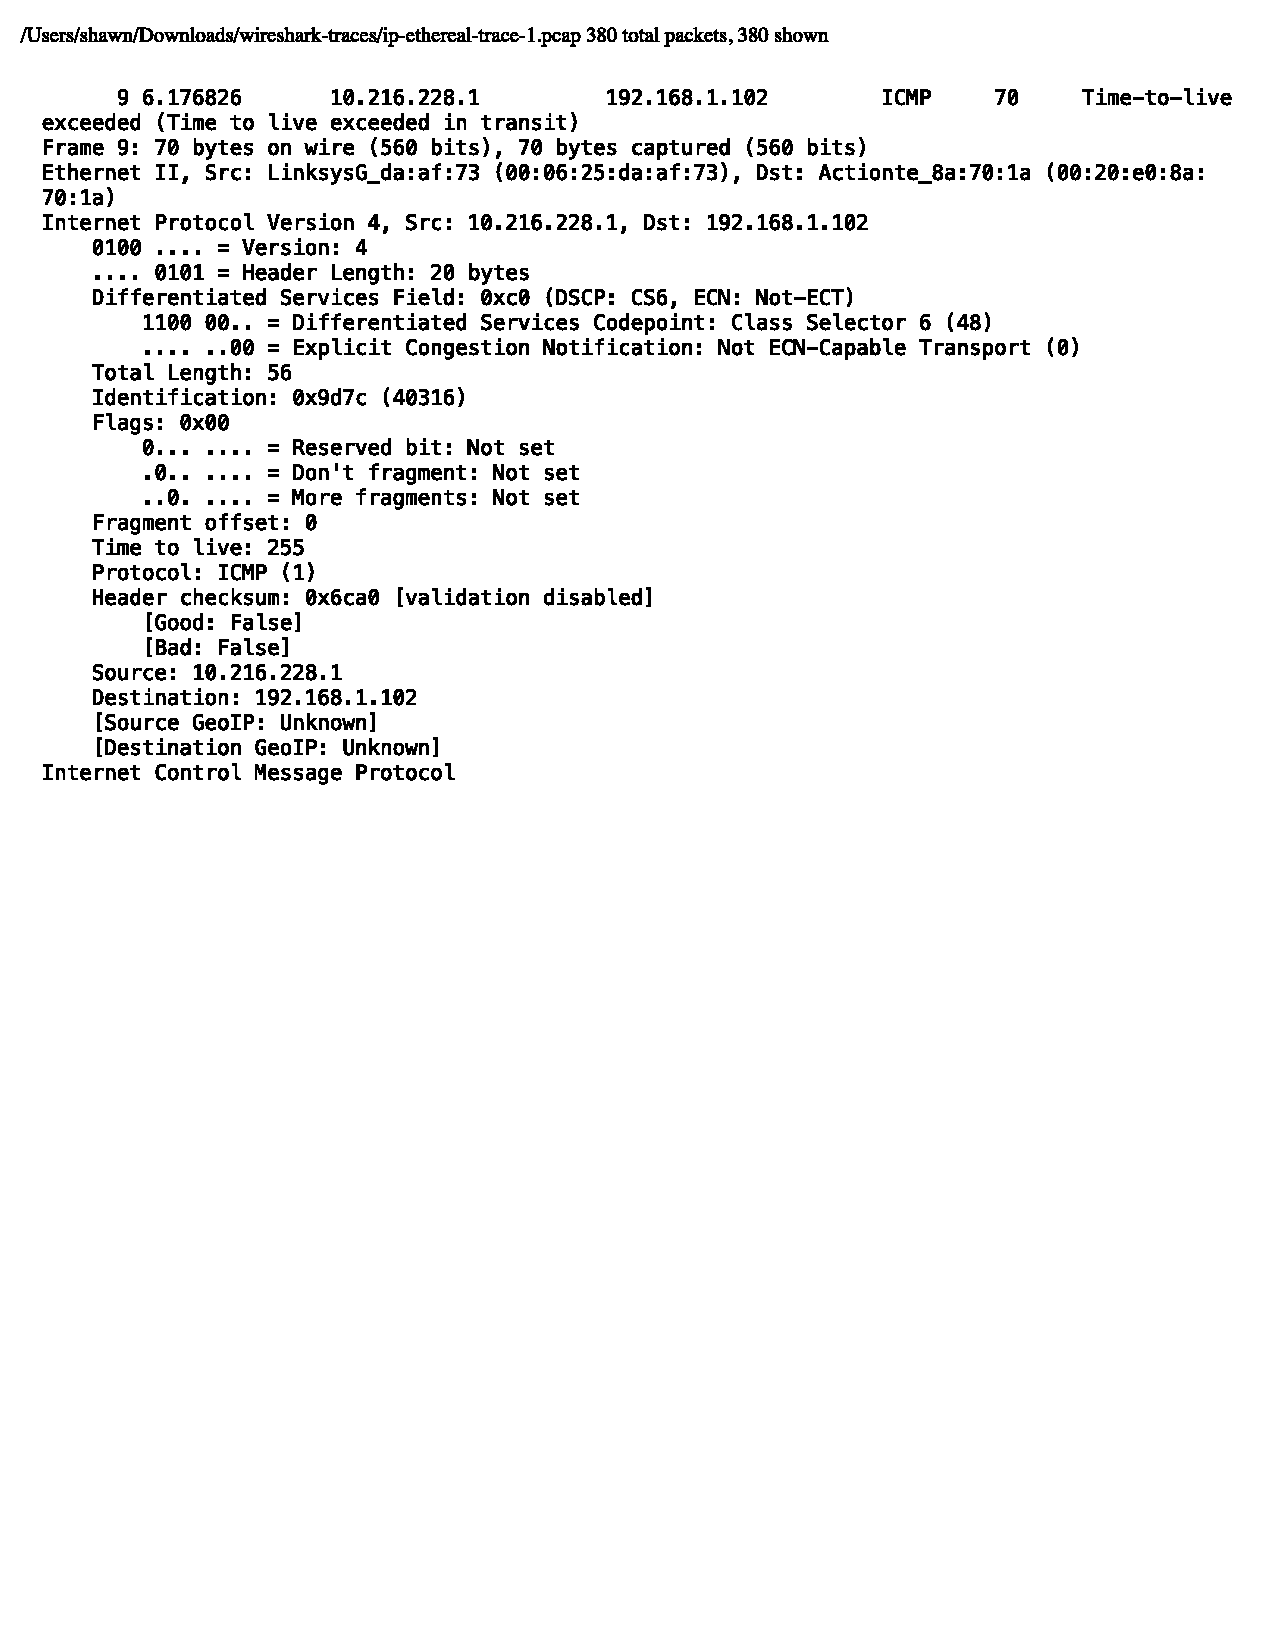
\includegraphics[width=\textwidth]{images/lab2-q8.pdf}
    \caption{ICMP Echo Reply}
    \label{fig:ip-icmp}
\end{figure}
According to figure \ref{fig:ip-icmp}, the identification is 40316 and TTL is 255. \\

\subsection*{Question 9}
Identification will change for every TTL-exceeded message but TTL remains the same. Because idetification is used to identify different pairs of ICMP packets, if they are the same, those packets will be considered as fragments of a large IP packet. TTL remains the same because it is from the same router. \\

\subsection*{Question 10}
\begin{figure}[!ht]
    \centering
    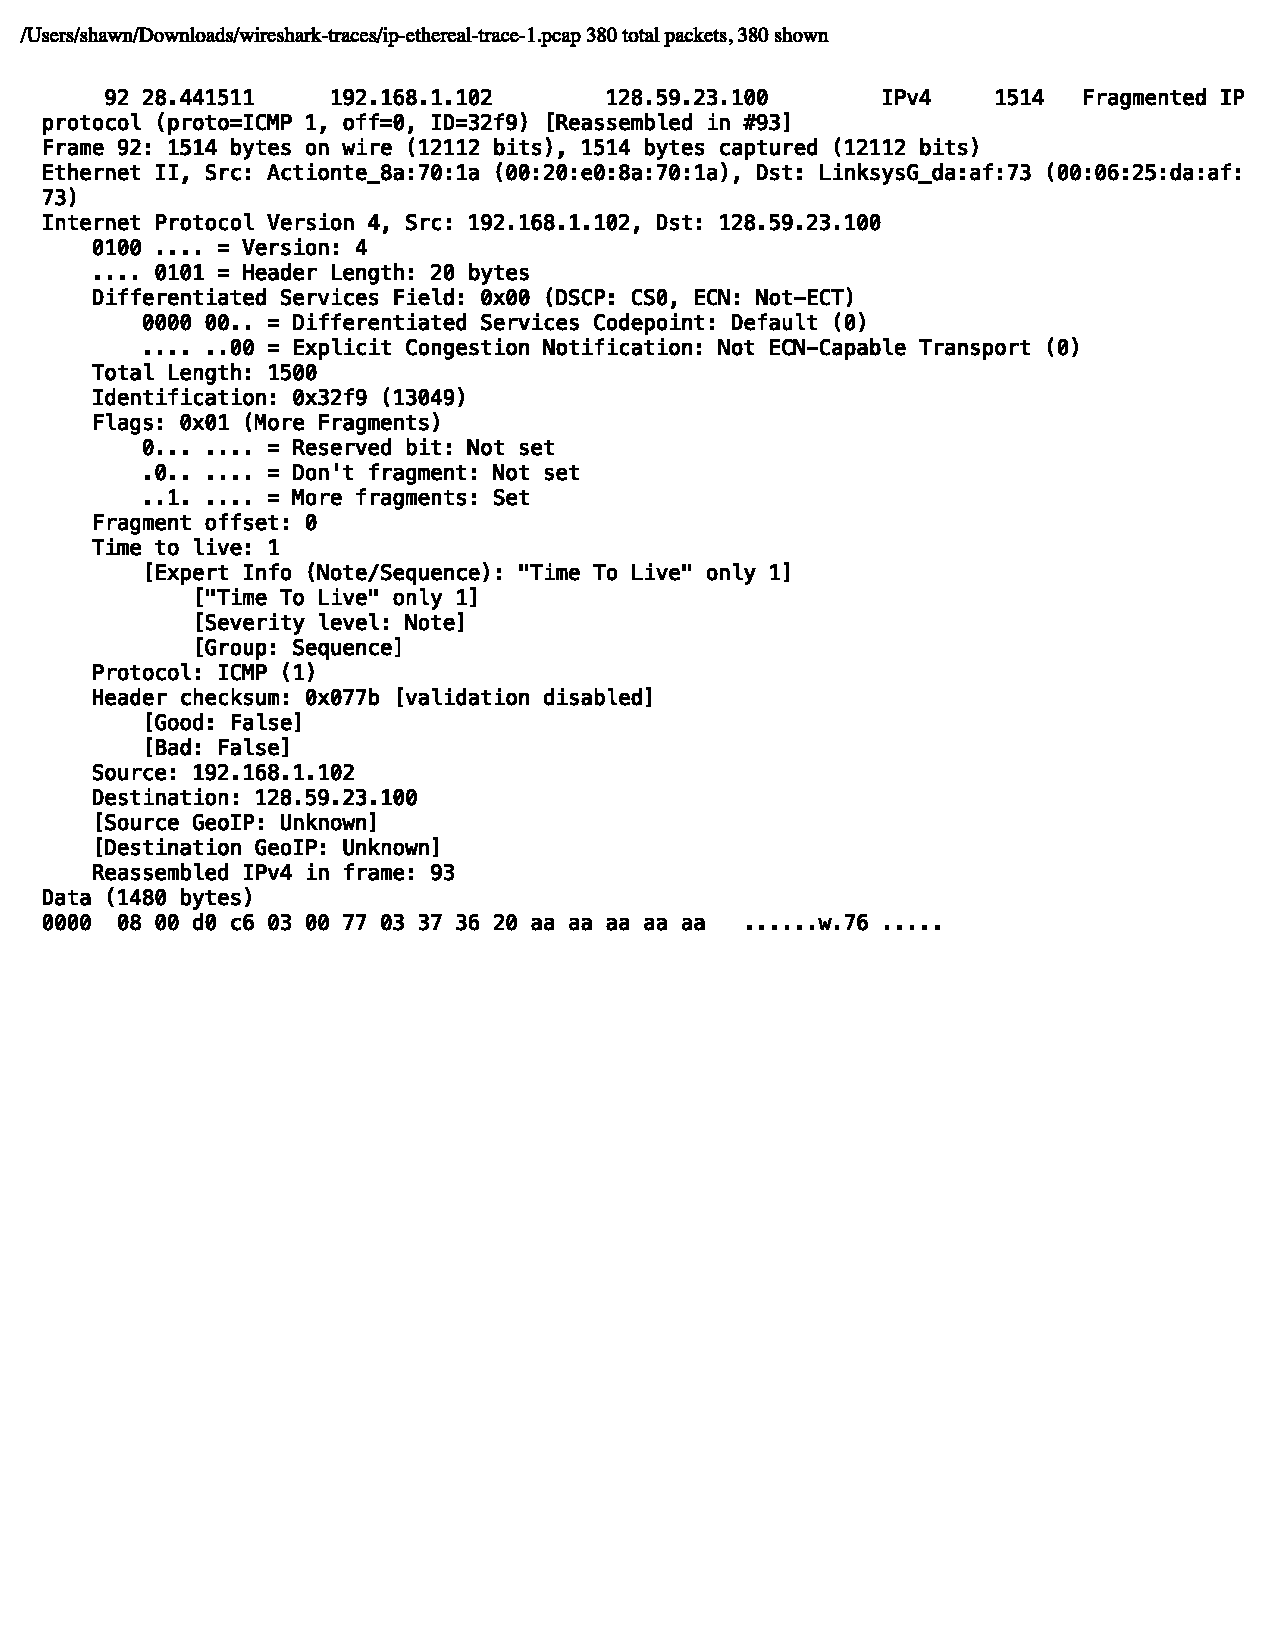
\includegraphics[width=\textwidth]{images/lab2-q10.pdf}
    \caption{ICMP Echo Reply (2000-byte)}
    \label{fig:ip-icmp2000}
\end{figure}
According to figure \ref{fig:ip-icmp2000}, yes, it is fragmented. \\

\subsection*{Question 11}
The more fragments bit in the flags field is set to 1, which indicates so. The fragment offset is 0 means this is the first fragment. This datagram is 1500 bytes in total. \\

\subsection*{Question 12}
\begin{figure}[!ht]
    \centering
    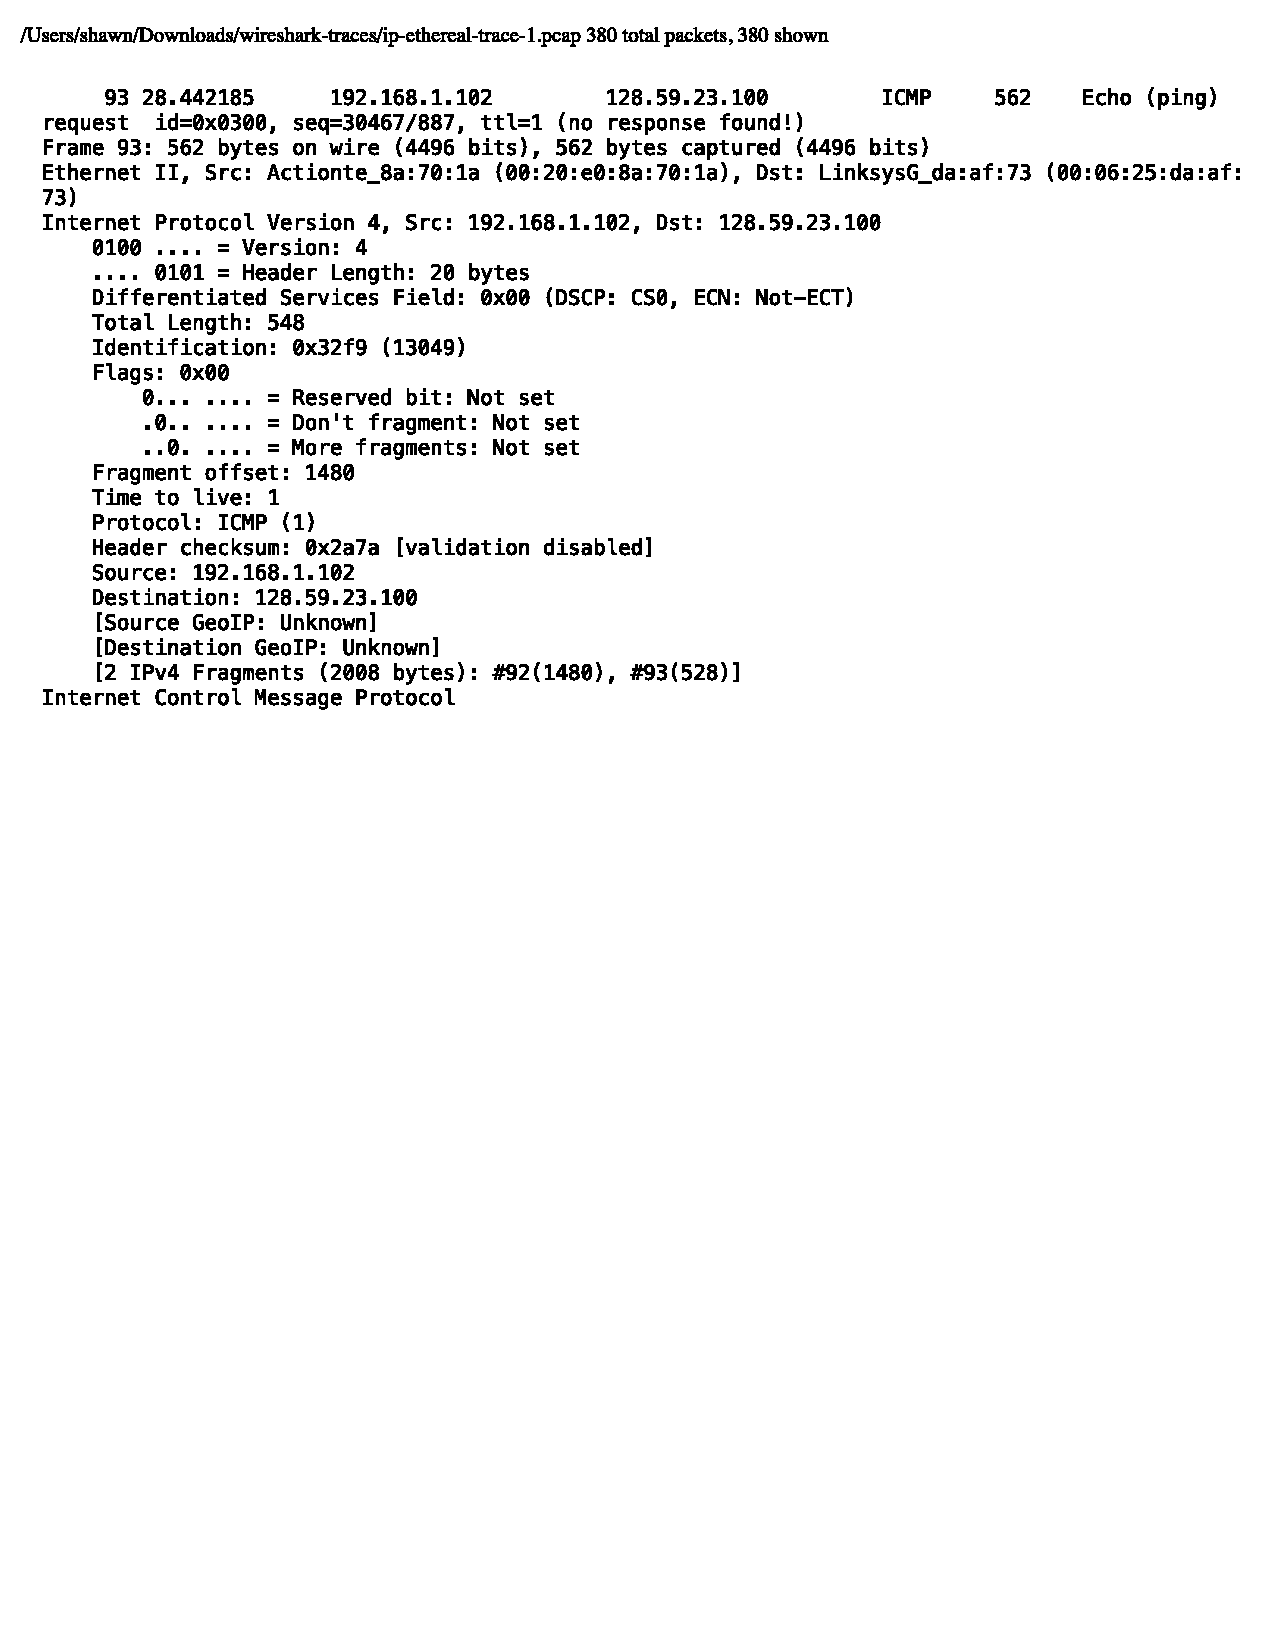
\includegraphics[width=\textwidth]{images/lab2-q12.pdf}
    \caption{ICMP Fragment}
    \label{fig:ip-fragment}
\end{figure}
According to figure \ref{fig:ip-fragment}, the fragment offset is 1480, which indicates it is not the first fragment. There are no more fragments because the more fragment bit is set to 0. \\

\subsection*{Question 13}
Total length, flags, fragment offset and checksum have changed. \\

\subsection*{Question 14}
\begin{figure}[!ht]
    \centering
    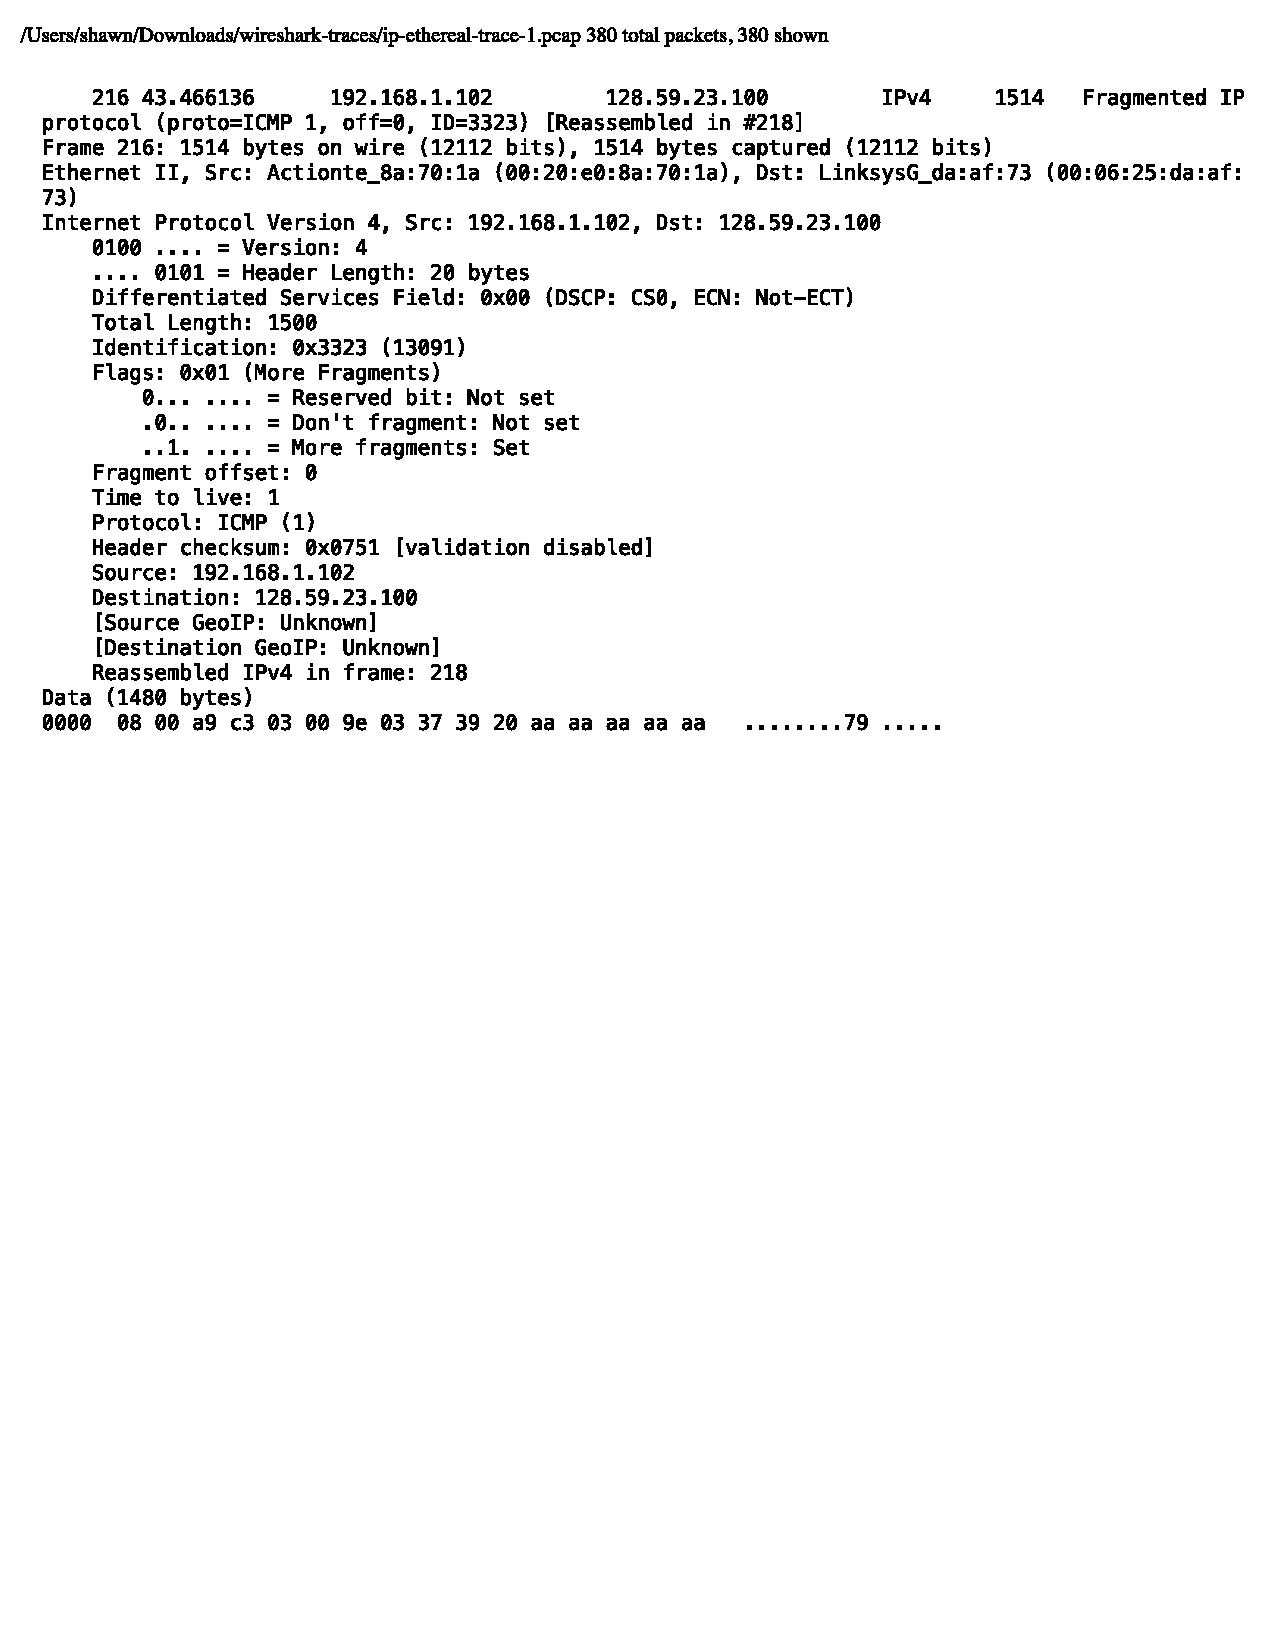
\includegraphics[width=\textwidth]{images/lab2-q14.pdf}
    \caption{ICMP Fragment (3500-byte)}
    \label{fig:ip-fragment3}
\end{figure}
According to figure \ref{fig:ip-fragment3}, 3 fragments are created. \\

\subsection*{Question 15}
The first and second fragment are different in fragment offset and checksum. The third is different from the previous two in total length, flags, fragment offset and checksum. 



\end{document}
